\section{Performances and Limitations}
\label{sec:performances_and_limitations}

Now that we have defined the core concept and individual components of a CSAC, we can proceed evaluating its performance and limitations using the metrics defined in Section \ref{sec:objective_metrics}.

In order to do so, we will consider and analyze the main disturbances effects that affect the overall performances, see what are the current solutions proposed and what they imply in terms of limitations and trade-offs.

\begin{figure}[H]
    \centering
    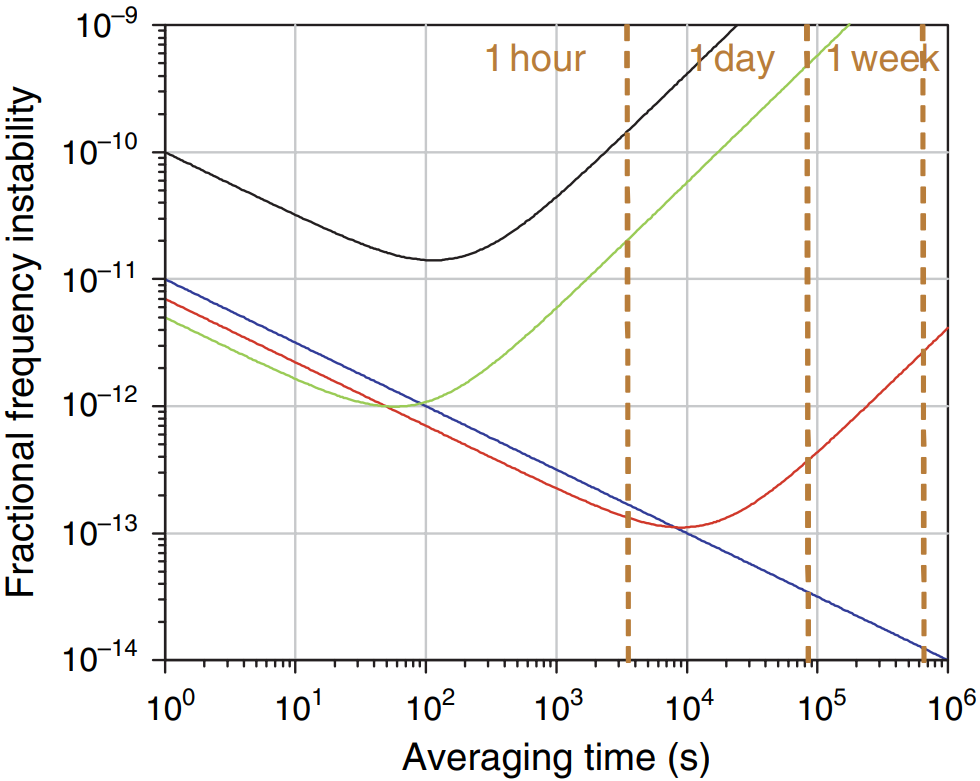
\includegraphics[width=0.6\textwidth, max width=\linewidth]{img/allan-deviation-graph.png}
    \caption{
        Allan deviation plot $\sigma_y(\tau)$ for different clock type sources
        (%
        \textcolor[HTML]{0000FF}{\acrfull{cs} Beam Standard},
        \textcolor[HTML]{FF0000}{\acrfull{rb} vapor cell clock},
        \textcolor[HTML]{00FF00}{Oven-controlled crystal oscillator (OCXO)},
        \textcolor[HTML]{000000}{Temperature-compensated crystal oscillator (TCXO)}%
        ). Source \cite{Knappe}.
    }
    \label{fig:allan_deviation_graph}
\end{figure}

In Figure \ref{fig:allan_deviation_graph}, it's visible a comparison of the Allan deviation $\sigma_y(\tau)$ for different clock sources.
Medium to long-term stability is represented, ranging from an average $\tau$ scale of $10^{0}$ to $10^{6}$ seconds, and is clearly visible how atomic clocks (both the Rb vapor cell and the Cs beam standard) outperform crystal oscillators in terms of stability.
However, it's important to notice that the Cs beam standard isn't a CSAC, but a traditional table-size atomic clock.
And also the Rb vapor cell clock represented in the plot is a Miniature Atomic Clock (MAC), which is larger and more power-hungry than a CSAC.
Typically, a CSAC is expected to have a stability $\sigma_y(\tau=1s) \approx 10^{-10}$, and the flicked floor at around $\tau = 10^4s$, positioning itself in between the TCXO and the OCXO in the short to medium-term stability range and outperforming them in the medium to long-term stability range.

\subsection{Short-term frequency stability}
\label{subsec:short_term_stability}

Short-term stability is strictly related to the Fast Noise of the local oscillator.

It's usually referred to very small time scale, in the order of $\tau < 1s$, and most of the time is not of real importance for real-world applications, where the main focus is on the medium and long-term stability.
However, in some particular cases, such as scientific experiments at the nanosecond scale, the short-term stability can be a key factor to consider.

Generally, we can expect to have a stability of $10^{-11} \le \sigma_y(\tau=1s) \le 10^{-10}$.

The most straightforward way to mitigate the Fast Noise is to improve the quality of the local oscillator (i.e. going from a TCXO to an OCXO), but this implies an increase in the power consumption and the size of the clock, which is not always possible in portable applications.

Another possibility would be to increase the frequency of the local oscillator, but then an appropriate frequency dividers would be required to obtain an output in the common electronic frequency range ($10Mhz$), increasing the overall size of the clock.

\subsection{Medium-term frequency stability}
\label{subsec:medium_term_stability}

Medium-term stability, instead, is one of the key metrics for all the applications where a CSAC is used.

It can be computed as stated in Equation \ref{eq:allan_deviation_medium} and is governed mostly by the stability of atomic interactions and energy levels.
Many factors can affect this type of stability, such as temperature of the environment, magnetic field, and quality of the excitation source.

Generally, we can expect to have an increasing stability from $10^{-10} @ \tau=1s$ to $10^{-12} @ \tau=10^4s$.
However, medium-term stability is strictly dependent on the quality of the physics package, its components and the design choices made to mitigate the disturbances.
The main disturbances together with some possible solutions (that always imply trade-offs) are listed below.


\paragraph{Rubidium vs. Cesium}

As we have seen, both \acrshort{rb} and \acrshort{cs} can be used as the atomic element inside the reference cell of a \acrshort{csac}.

However, it has to be noted that the splitting gap in the two hyperfine ground levels is not the same for the two elements.
In fact, comparing \ref{itm:Rb-I} and \ref{itm:Cs-I} transitions, we can see that the frequency of the \acrshort{rb} transition is around $6.8GHz$, while the \acrshort{cs} transition is around $9.2GHz$.
By recalling Equation \ref{eq:allan_deviation_medium} for the medium-term stability, we can observe that the stability is inversely proportional to the line quality factor $Q$.
Being $Q = \frac{\nu_0}{\Delta\nu}$, we can understand that the higher the frequency of the transition, the higher the stability of the clock.
So, in theory, a \acrshort{cs}-based clock should have a better stability than a \acrshort{rb}-based one.

On the other hand, the \acrshort{rb} has a simpler and easier to control pumping system that has a better coupling efficiency with the atomic resonance frequency with respect to the diode laser used in the \acrshort{cs} clock.

For this reason, the performance of the two clocks is quite similar, with the \acrshort{cs} clock being slightly better in terms of power consumption and size, but with a more complex and expensive physics package.


\paragraph{Gas pressure and composition inside the reference cell}

Collision with untreated interior walls of the reference cell can depolarize the spin of electrons, forcing them to return to the ground state.
For this reason, the signal in output from the Physical Package will be reduced ($SNR$ reduction) and also the medium-term stability will be affected.

To mitigate this effect, the reference cell is usually filled with a precise combination of gases, such as Helium, Neon, Argon or Nitrogen.
Those gasses help in reducing the number of collisions of the Rubidium or Cesium atoms with the inner wall, enhancing the possibility of electrons to remain in the excited state for a longer time, increasing the signal-to-noise ratio $SNR$.

However, we know that the gas pressure inside the reference cell depends also on the temperature.
For this reason, the temperature of the reference cell must be kept constant to ensure a stable gas pressure and composition.
This is also done via a dedicated servo loop as explained in Section \ref{subsec:control_loop}.
However, the use of a dedicated thermo-stabilizing system implies an increase in both the power consumption and the size of the clock.


\paragraph{Quality of the excitation source}

Another key factor that can affect the stability of the CSAC is the quality of the excitation source.

Both the bulb lamp and the diode laser are dependent from the temperature.
A small variation in frequency can reduce the coupling between the excitation source and the atomic resonance frequency, affecting the medium-term stability of the clock.
For this reason, the temperature of the laser source must be tuned accordingly by an appropriate servo loop.

If we consider a VCSEL source (as in the case of a CPT-based clock), the temperature sensibility is around $300 GHz/K$, which means that even a very small temperature variation can greatly shift the frequency of the laser source, reducing the number of electrons in the dark state, thus decreasing the signal-to-noise ratio $SNR$.


\paragraph{Magnetic field (Zeeman effect)}

The presence of an external magnetic field can also significantly affect the accuracy of the CSAC.

The Zeeman effect is a phenomenon that splits the atomic energy levels into multiple sublevels when an external magnetic field is applied.
By doing so, the atomic resonance frequency is shifted, affecting the accuracy of the clock.
In particular, the magnitude of the Zeeman shift is proportional to the strength of the magnetic field applied.

To mitigate this effect, the entire physics package is usually shielded with a magnetic shield to reduce the impact of the external magnetic field on the atomic transitions.
In some cases, the CSAC can also have an internal magnetic field, called \textit{C-field}, to counteract the external one.
If that is the case, an appropriate control loop is adopted to minimize the disturbance effect.

Moreover, by applying a known magnetic field to the physics package, the Zeeman shift can be measured and used to precisely calibrate the clock.


\paragraph{Optical instabilities (Stark effect)}

Similarly to the Zeeman effect, the Stark effect can also shift the atomic energy levels, affecting the accuracy of the clock.

The Stark effect is a phenomenon that occurs when an oscillatory external electric field interacts with the charged nucleus and electrons within the atom, modifying their energy.
In case of a CSAC, the excitation photon might be subjected to instabilities in intensity and/or spectral profile, inducing unintended Stark shifts that can cause deviations in the atomic resonance frequencies, leading to clock frequency instability.

% To mitigate this effect, the excitation source must be carefully designed and controlled.
% In some cases, it's possible to opt for a pulsed excitation instead of a continuous one.
% In this way the Stark effect can be minimized, but on the other hand the signal-to-noise ratio will be reduced
% Usually a VCSEL has higher frequency noise than Rb lamp.


\paragraph{Frequency shifts (Doppler effect)}

Finally, a huge source of disturbance for the CSAC is the Doppler effect.

Inside the reference cell in fact, atoms are continuously moving with random directions.
In this way, even if the excitation frequency is carefully selected, a red or blue shift can occur depending on the atom velocity and the coupling between the source and the atomic resonance frequency can be reduced.
This implies a reduction in the signal-to-noise ratio and a decrease in the medium-term stability of the clock.

A proposed solution is to reduce the mean-free-path of the atoms, by reducing either the pressure or the temperature inside the reference cell.
However, in order to achieve this, more thermal power stabilization is required.

\subsection{Long-term frequency stability}
\label{subsec:long_term_stability}

Long-term stability refers to the ability of maintaining frequency accuracy over extended periods (hours, days or even months).

Here, all the previously mentioned disturbances can have a significant impact.
The aging of the components is also relevant and to be considered.
Over longer periods of time, the pressure inside the reference cell might change, the quality of the excitation source might degrade, and so also the mechanical properties of the local oscillator.

Temperature exposition is also a key factor in the long-term stability of the clock.
If excessive temperature is applied for long periods of time, the gas pressure inside the reference cell will increase and also the vacuum integrity of the entire clock would be affected.
Moreover, the electronics circuits degrade faster at higher temperatures, reducing the overall lifetime of the clock.

\subsection{Frequency Stability vs. Size, Weight, and Power (SWaP)}
\label{subsec:stability_vs_SWaP}

As we have seen in the previous paragraphs, a strong correlation exists between the stability of the clock and its size, weight, and power consumption.
To achieve better performances, a series of internal components must be increased in size (e.g. the reference cell) or quality (e.g. the local oscillator), or additional servo loops must be added to control the disturbances (and indeed more sensor and actuator are required).

So qualitatively, we can understand how better performances are associated with an increase in the SWaP of the clock.
In Figure \ref{fig:ADEV_vs_SWaP}, we can observe how the Allan deviation $\sigma_y(\tau=1s)$ is related to the SWaP of the clock for different types of atomic clocks, ranging from the traditional table-size atomic clock to the CSAC.

\begin{figure}[H]
    \centering
    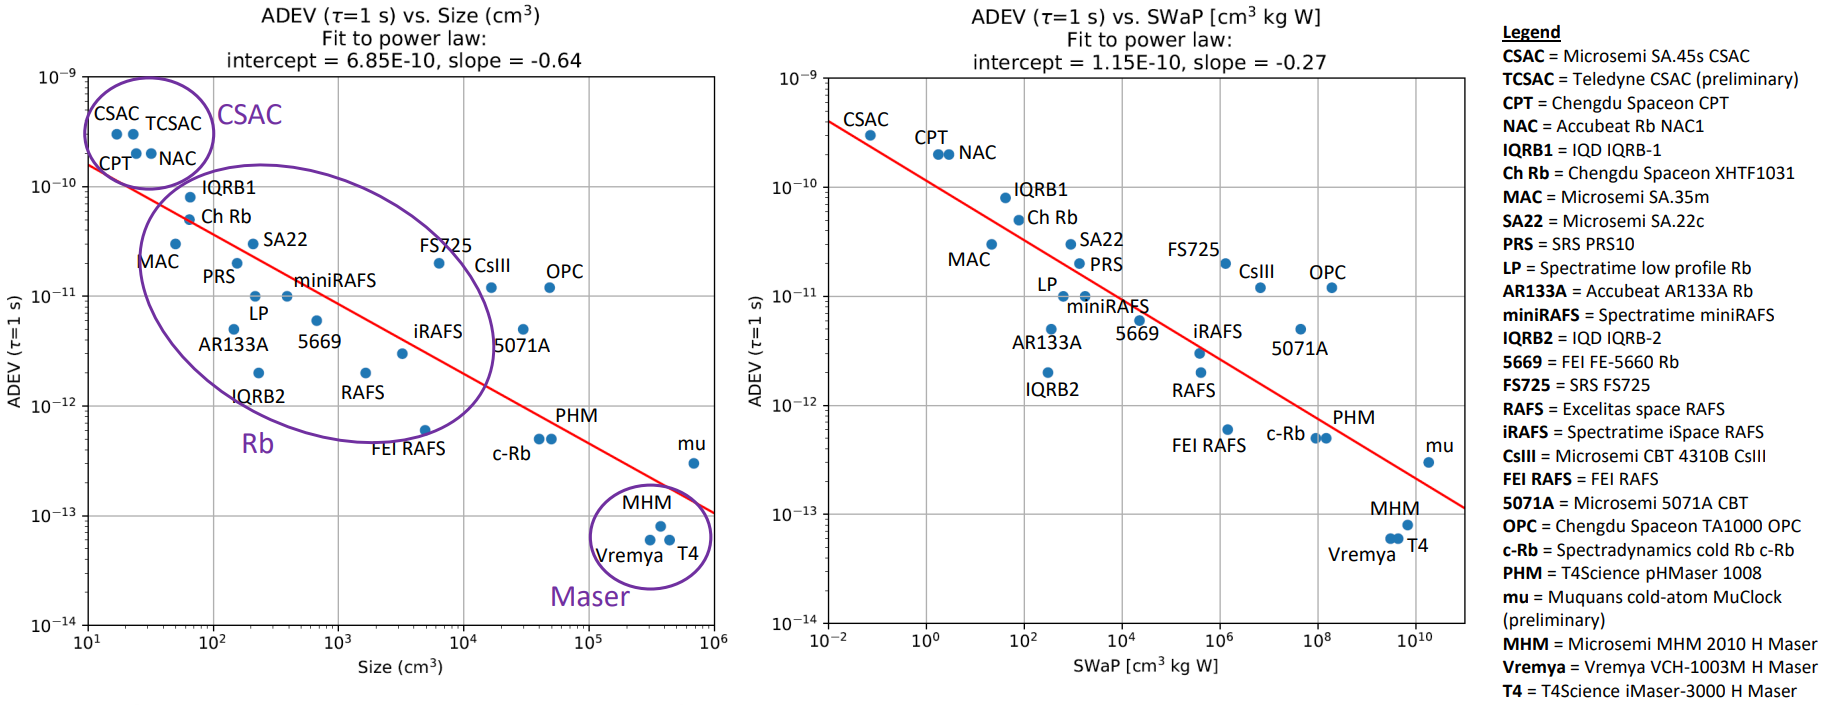
\includegraphics[width=\textwidth, max width=\linewidth]{img/ADEV_vs_SWaP.png}
    \caption{Allan deviation $\sigma_y(\tau=1s)$ vs. Size, Weight, and Power (SWaP) for different atomic clocks. Source \cite{Scherer}.}
    \label{fig:ADEV_vs_SWaP}
\end{figure}

As also marked by the red lines in both the plots, it's clear that a correlation exist and that is not possible to achieve a very high stability without a significant increase in the SWaP of the clock.
In particular, the equations of the two red lines are\footnote{The units adopted in the equations related to the SWaP are: Size and Volume $[cm^3]$, Weight $[kg]$, Power $[W]$}:

\begin{align}
    \sigma_y(\tau=1s) & = 6.85 \times 10^{-10} + \text{volume}^{-0.64} \\
    \sigma_y(\tau=1s) & = 1.15 \times 10^{-10} + \text{SWaP}^{-0.27}
\end{align}



